\rhead{8. Dijagrami sekvence}
\section{Dijagrami sekvence}
\par U nastavku se nalaze dijagrami sekvence korišćeni za analizu interakcija u sistemu. Opisana su 4 dijagrama sekvence:
\begin{itemize}
    \item \textbf{Promocija u volontera}
    \item todo
    \item todo
    \item todo
\end{itemize}
\subsection{Promocija u volontera}
\par Član može da postane \textit{volonter} tako što pošalje zahtev za volonterstvo. Svaki \textit{volonter} može da glasa samo jednom dokle god traje glasanje. 
Na kraju glasanja, status zahteva se menja u zavisnosti od broja glasova. Da bi zahtev bio prihvaćen,
potrebno je da 50\% glasača budu za promociju. Ukoliko je zahtev prihvaćen članu se menja status. Ovo je prikazano na slici \ref{fig:promotion-seq}.
\begin{figure}[h]
    \centering
    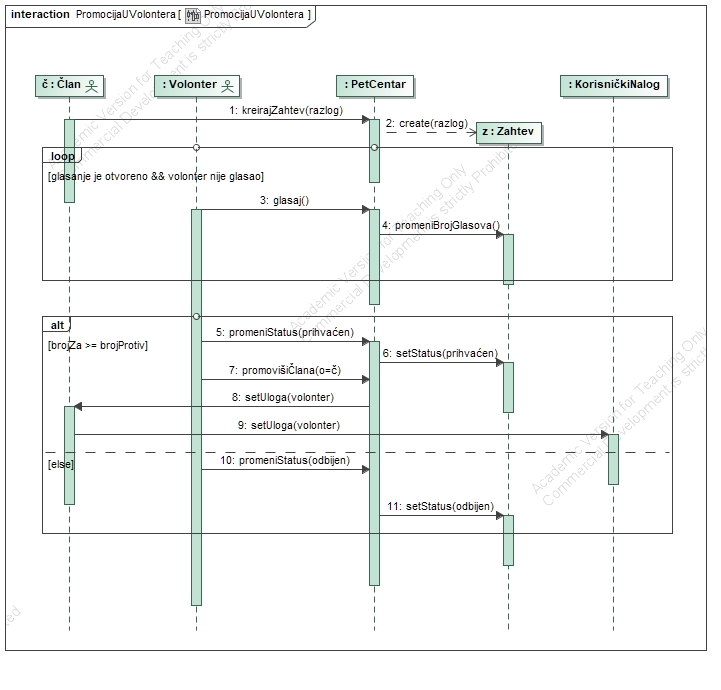
\includegraphics[width=\textwidth, height=0.9\textwidth]{img/promote-member-sequence.jpg}
    \caption{Promocija u volontera}
    \label{fig:promotion-seq}
\end{figure}